% generated by laprint.m
%
\begin{psfrags}%
\psfragscanon%
%
% text strings:
\psfrag{s05}[rt][rt]{\fontsize{10}{15}\fontseries{m}\mathversion{normal}\fontshape{n}\selectfont \color[rgb]{0,0,0}\setlength{\tabcolsep}{0pt}\begin{tabular}{r}$\sigma^{-1}=1.1$\end{tabular}}%
\psfrag{s06}[][]{\fontsize{10}{15}\fontseries{m}\mathversion{normal}\fontshape{n}\selectfont \color[rgb]{0,0,0}\setlength{\tabcolsep}{0pt}\begin{tabular}{c}$\phi$\end{tabular}}%
\psfrag{s07}[][]{\fontsize{10}{15}\fontseries{m}\mathversion{normal}\fontshape{n}\selectfont \color[rgb]{0,0,0}\setlength{\tabcolsep}{0pt}\begin{tabular}{c}$\hat{z}_f$\end{tabular}}%
%
% axes ticklabel color:
\color[rgb]{0.15,0.15,0.15}%
%
% axes font properties:
\fontsize{10}{15}\fontseries{m}\mathversion{normal}%
\fontshape{n}\selectfont%
%
% xticklabels:
\psfrag{x01}[t][t]{0}%
\psfrag{x02}[t][t]{0.25}%
\psfrag{x03}[t][t]{0.5}%
%
% yticklabels:
\psfrag{v01}[r][r]{0}%
\psfrag{v02}[r][r]{0.25}%
\psfrag{v03}[r][r]{0.5}%
\psfrag{v04}[r][r]{0.75}%
\psfrag{v05}[r][r]{1}%
%
% Figure:
\resizebox{16cm}{!}{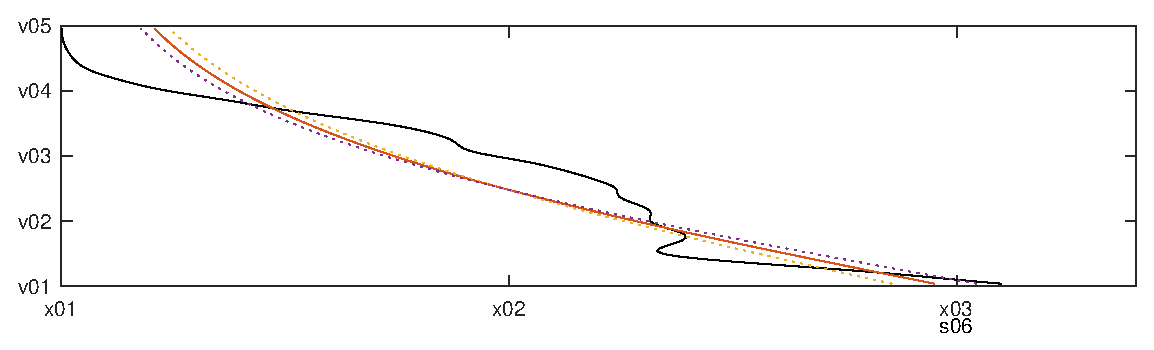
\includegraphics{phifitall_topcut.matlab.eps}}%
\end{psfrags}%
%
% End phifitall_topcut.matlab.tex
